%
% File eamt11.tex, adapted from eamt10.tex
%
% Contact: vincent@ccl.kuleuven.be

%%% To ease future customizations, various replaceables have been paramaterized
%%% as listed in the newcommands section

\documentclass[11pt]{article}
\usepackage[utf8x]{inputenc}
\usepackage{eamt11}
\usepackage{url}
\usepackage{times}
\usepackage{multirow}
\usepackage[afrikaans,dutch,english]{babel}
\usepackage[small,bf]{caption}
\usepackage{latexsym}
\usepackage{graphicx}
\usepackage{gb4e}
\usepackage{linguex} %think it has to be the last package

\setlength\titlebox{6.5cm}    % Expanding the titlebox

\newcommand{\confname}{EAMT 2011}
\newcommand{\website}{http://www.eamt2011.eu/}
\newcommand{\contactname}{the programme chairs Mikel Forcada \& Heidi De Praetere}
\newcommand{\contactemail}{mlf@dlsi.ua.es} 
\newcommand{\conffilename}{eamt11}
\newcommand{\downloadsite}{http://www.eamt2011.eu/}
\newcommand{\paperlength}{$8$ (eight)}
\newcommand{\shortpaperlength}{$4$ (four)}

\title{Rapid rule-based machine translation between Dutch and Afrikaans}

\author{Pim Otte\\
  Mendelcollege\\
  Pim Mulierlaan 4\\
  2024 BT Haarlem\\
  {\tt 5666@mendelcollege.nl}  \And
  Francis M. Tyers\\
  Dept. Lleng. i Sist. Inform.\\
  Universitat d'Alacant\\
  E-03070 Alacant \\
  {\tt ftyers@dlsi.ua.es}}

\date{}

\begin{document}
\maketitle
\begin{abstract}
 This paper describes the design, development and evaluation of a machine
 translation system between Dutch and Afrikaans developed over a period of
 around a month. The system relies heavily on the re-use of existing 
 publically available resources such as Wiktionary, Wikipedia and the 
 Apertium machine translation platform.
\end{abstract}

\section{Introduction}

Dutch is a West-Germanic language spoken by nearly 23 million people, 
mostly from the Netherlands and Flanders, the Dutch-speaking part of Belgium and a minority 
living in former colonies of the Netherlands, such as Suriname, Aruba and the Netherlands 
Antilles. Dutch, as it is today, started developing in the 16th century in the 
major trade cities, such as Amsterdam and Antwerp \cite{Shetter:02}.  Afrikaans is spoken 
by at least 5 million people, mainly in South Africa but also in Namibia. Afrikaans is a 
variety of Dutch that originates from that spoken by the Dutch colonists of 
the Cape Colony. In 1925 Afrikaans replaced Dutch as an official language in South Africa, to 
be the joint official language together with English. \cite{Donaldson:93} Currently, Afrikaans is one of the 
eleven national languages. 

In this paper we will describe the development of {\small {\tt apertium-af-nl}}, a bi-directional Afrikaans 
and Dutch machine-translation system based on the Apertium platform. As Afrikaans and Dutch 
are largely mutually intelligible, this machine translation system focuses on dissemination, the 
translation of text for the purpose of being post-edited and then being published. 

This is not the first system to work with this language pair, \newcite{Huyssteen:09} describe
a rule-based system to convert in a single direction from Dutch to Afrikaans. 
The reason we have chosen to work with a rule-based approach, instead of the ubiquitous 
corpus-based/statistical approach, is that the latter needs parallel corpora for the two 
languages. The only freely available Afrikaans--Dutch corpus, is 
KDE4\footnote{\url{http://opus.lingfil.uu.se/KDE4.php}}, which is translated via English and 
domain specific. We feel that these corpora do not approach the quality required for the
statistical approach, and the fact that Afrikaans and Dutch are closely related languages 
makes a rule-based approach favourable.

The paper is laid out as follows: firstly, we will describe the reuse and creations of 
resources. We will then discuss several grammatical features of Afrikaans and Dutch and how 
these were treated in the machine-translation system. We will then present a section 
in which the system is evaluated. Finally, we will discuss the system and future work that 
could be done.

\section{Method}

The system is based on the Apertium machine translation platform.\footnote{\url{http://www.apertium.org}} The
platform was originally aimed at the Romance languages of the Iberian
peninsula, but has also been adapted for other, more distantly related,
language pairs. The whole platform, both programs and data, are licensed
under the Free Software Foundation's General Public
Licence\footnote{\url{http://www.fsf.org/licensing/licenses/gpl.html}} (GPL)
and all the software and data for the 25 supported language pairs (and the
other pairs being worked on) is available for download from the project
website.

\begin{figure*}
  \centering
  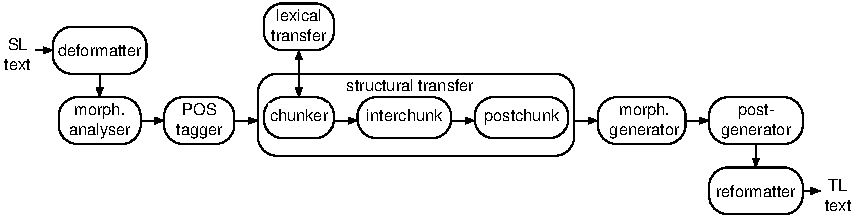
\includegraphics[scale=0.8]{apertium2.pdf}
  \caption{Modular architecture of the Apertium MT
    platform. The compound analysis and generation modules are included at the morphological
    analyser and morphological generator stages respectively.}
\label{fg:apertium}
\end{figure*}

{\small {\tt apertium-af-nl}} has been developed over the course of one and a half months.
The vast majority of the work has been done by a Dutch secondary school student supervised 
by a PhD student. However, since for the latter this was not paid and for the former it was not for school, there were 
very few full 8-hour days of work during this period.

\subsection{Existing resources}

One existing resource was reused with very little modification: the 
morphological transducer for Afrikaans, which was created during a separate, currently dormant, 
project on English--Afrikaans machine translation. However, some changes were made. The structure 
of verb entries was wholly revised, and both infrequent words and words for which a translation
could not be found, were removed.

\subsection{Resources created}

\subsubsection{Dutch morphological transducer}

There are a number of existing morphological analysers for Dutch \cite{Bosch:07,Laureys:04,DePauw:04},
some of which also function as morphological generators. Our decision to make a new morphological 
analyser was based on the following rationale:

\begin{itemize}
\item Licence: Neither the CELEX morphological database for Dutch \cite{Laureys:04},
    nor the finite-state morphological transducer in the FLaVoR project \cite{DePauw:04}
    are available under a free licence. As our objective is to publish and distribute 
    the system described here, this made them unusable.
\item Bidirectional: We wanted the dictionary to be able to be used for both
    morphological analysis and generation. Other analysers, for example the 
    one described in \newcite{Bosch:07} are only designed for analysis.
\item Tagset: When creating a new machine translation system, it is convenient
    if the tags which represent the same or similar features are equivalent in the 
    morphological analysers/generators for each of the languages,
    e.g. {\small {\tt $<$sg$>$}} on both sides for `Singular' instead 
    of {\small {\tt $<$sg$>$}} on one side and {\small {\tt ev}} 
    \footnote{{\tt ev} stands for \emph{enkelvoud} `singular' and is from the tagset of the Tadpole morphological analyser.} on the other.
\end{itemize}

The open categories (nouns, verbs, adjectives, adverbs) for the Dutch 
morphological analyser were extracted semi-automatically from 
Wiktionary,\footnote{\url{http://www.wiktionary.org}} a free online, multilingual
dictionary that often includes inflectional information. On the English Wiktionary, in the case 
of Dutch nouns it often (although not always) gives the gender and the 
plural and diminutive forms (see for example Figure~\ref{fig:wikt1}).
The category {\small {\tt Dutch nouns}} in the English Wiktionary has a total of 10,610 entries,
while the corresponding category on the Dutch Wiktionary has 13,176 entries.

Closed categories were added by hand based on a grammar of Dutch \cite{Shetter:02}.

\begin{figure}
\centering
\begin{tiny}
\begin{tabular}{|l|}
\hline
{\large Dutch} \\
~\\
{\bf Etymology}\\
~\\
~{\em hoofd-} (``main, head'') + {\em stad} (``city'')\\
~\\
{\bf Pronunciation}\\
~\\
{\bf Noun}\\
~\\
{\bf hoofdstad} m. ({\em pl} hoofdsteden, {\em dimin} hoofdstadje, {\em dimin pl} hoofdstadjes) \\
~\\
~~~~1. capital city \\

\hline
\end{tabular}
\end{tiny}
\caption{English language Wiktionary article for Dutch \emph{hoofdstad} `capital city' 
    {\small \url{http://en.wiktionary.org/wiki/hoofdstad}}}
\label{fig:wikt1}
\end{figure}

\subsubsection{Bilingual dictionary}

The bilingual dictionary has been developed in several ways.
Exact matches from the dictionaries
were automatically added to the bilingual dictionary. Proper names were added in the
way that is described in \newcite{Tyers:08}. After that cognates were added. There are several
small common spelling differences between Afrikaans and Dutch. For example,
where the letter `y' in Afrikaans is used, Dutch often uses the digraph `ij'.
The bilingual dictionary was expanded further by categorising these spelling differences and
automatically adding translations to the bilingual dictionary if the spelling difference was the
only difference between the two words. Finally, some entries were done by hand.
This included closed categories, but also words that frequently appeared in Wikipedia
which were not yet in the bilingual dictionary.

\subsection{Transfer rules}

A total of 32 transfer rules have been written for the direction Afrikaans$\rightarrow$Dutch and
15 for the direction Dutch$\rightarrow$Afrikaans. Some of these transfer rules are discussed 
below.

\subsubsection{Afrikaans to Dutch}

%%Dutch cannot use the present tense in past situations (not even in narrative style)

Afrikaans hardly uses the word-attached genitive \cite{Donaldson:93} \emph{s}. The word \emph{se} is used to indicate possesion. 
Therefore, a transfer rule has been added to remove the \emph{se} and instead make the preceding
noun genitive. Note that in Dutch the genitive is not the preferred translation. A construction using
the word \emph{van} `of' would be preferable, but would need restructuring of the phrase. 

%af:Die vrou se seun.
%nl:De vrouws zoon.
%gloss:DEF.ARTICLE woman.NOUN.GEN son.NOUN

The verb \emph{hê} `have' is the only verb used in Afrikaans as auxiliary
verb with a past participle. In Dutch the verbs \emph{hebben} `have' and \emph{zijn} `be' 
are both used, the latter mostly in cases of movement and a few exceptional cases, the
former in all others. To handle this, two transfer rules have been added, to handle the
patterns `hê + past participle' and `hê + nie + past participle + nie', which change the
verb to have into the verb to be, when the past participle is found in a list of verbs that go with
`zijn'.

%af:Ek het geval.
%nl:Ik ben gevallen.
%gloss: PERSPRNSUBJ.P1.SG have.VERB fallen.PP

% \item Concordance of article and complement

Nouns in Afrikaans do not exhibit gender, where nouns in Dutch can be one of four genders,
neuter, masculine, feminine or common. The definite article \emph{het}, \emph{die} in Dutch must agree with 
the noun it modifies. A number of transfer rules were written for patterns such as `determiner + noun',
`determiner + adjective + noun', etc., which propagate the gender of the head noun to the article.

\begin{itemize}
\item Concordance between subject and verb
\item Removal of negation scope marker
\end{itemize}

\begin{itemize}
\item Addition of negation scope marker
\end{itemize}


\subsubsection{Compound words}

%% give some statistics for what percentage of words are compounds in dutch/afrikaans
%% give some justification for only doing noun-noun compounds (e.g. more frequent, easier to identify??)

Both Afrikaans and Dutch are languages in which words combine very
productively into compounds. For example the words {\em infrastruktuurontwikkelingsplan}
`infrastructure development plan' and {\em lugmagbasis}
`air force base'. As it is impractical to introduce
all compound words into the lexicons, compound word analysis is performed on
all unknown words. The analysis process works longest-match left-to-right
using the same transducer as is used for morphological analysis. This process only
looks for compounds made up of just nouns, because they are more frequent than other compounds.
Results are restricted by two special
symbols which do not appear in the output {\small {\tt compound-L}} and {\small {\tt compound-R}}.
The {\small {\tt compound-L}} symbol is used for forms that can only appear on the
left side (e.g. surface form) of a compound, where {\small {\tt compound-R}} is
used for forms that can either appear in a compound, or end it.
Epenthetics, that is linking letters that occur between compound words,
are also taken care of heuristically in this way. For example the -s-
in \emph{ontwikkelingsplan}, the -en- in \emph{pannenkoek} and the -e- in \emph{paardebloem}.
Notice that the epenthetic -e- is not productive in Dutch, that is, it is not used 
in new compounds.

%\begin{figure*}
%\begin{small}
%\begin{verbatim}
%die lugmagbasis
%
%^die<det><def><sg>$
%^lug<n><sg><cmp>+mag<n><sg><cmp>+basis<n><sg>$
%
%^de<det><ind><mf><sg>$
%^lucht<n><mf><sg><cmp>$^macht<n><mf><sg><cmp>$^basis<n><f><sg>$
%
%de luchtmachtbasis
%\end{verbatim}
%\end{small}
%\end{figure*}

There are some limitations to this method. For example: although
both {\em macht-} and {\em machts-} can be analysed as an internal part
of a compound, only one of them can be generated. Which one will be generated
is decided based on the inflectional paradigm to which the word belongs. For
example {\small {\tt ontwikkeling$<$n$><$sg$><$cmp$>$}} will always produce {\em ontwikkelings-} in generation,
where {\small {\tt macht$<$n$><$sg$><$cmp$>$}} will always produce {\em macht-}.

\subsubsection{Separable verbs}

Another feature of Afrikaans and Dutch is separable verbs, for example
the word {\em afslaan} `to turn, to decline, to stop'. This can appear in the following
forms {\em afslaan}, {\em sla af}, {\em afgeslagen}. Additionally the two constituent
parts of the verb in {\em sla af}, the verb itself {\em sla} and the particle
{\em af} may be separated by a word or phrase, {\em Ik sla het aanbod af.}
 `I decline the offer'.

The following cases are supported,

\begin{itemize}
\item Infinitive: afslaan $\rightarrow$ afslaan 
\item Participle: afgeslagen $\rightarrow$ afgeslaan
\item Non-separated: Ik sla af naar rechts. $\rightarrow$ Ek slaan af na regs
\item Subordinate: Toen ik de bal afsloeg $\rightarrow$ Toe ek die bal afslaan
\end{itemize}

Verbs separated by a word or phrase are currently translated word-for-word,
so the particle and verb are translated. This causes a problem when the
verb is not constructed equally in Afrikaans and Dutch. Also, when one part
of the verb, does not exist as a stand-alone verb, it is not recognised by the analyser.
for example in {\em aankondig} `to announce' {\em kondig} is not a word. Thus {\em ... kondig ... aan} 
cannot be analysed currently.

A module is under development to handle separable verbs, but is currently
in the prototype stage.

There are currently 484 separable verbs defined in the bilingual
dictionary. Of these, 439 are separable in both languages, 33 are
separable in Afrikaans but not in Dutch, and 12 are separable in
Dutch but not Afrikaans.

\subsection{Current status}

In terms of dictionary entries, the pair currently has 7,258 entries in the Afrikaans
morphological dictionary, 7,048 in the Dutch morphological dictionary and 5,982 in the 
Bilingual dictionary.

\section{Evaluation}

The system was evaluated in five ways. The first was the 
coverage\footnote{Here coverage is defined as \emph{na\"ive coverage}, 
that is for any given surface form at least one analysis is returned. This 
may not be complete.} of the system. The second was an evaluation of the 
compound analysis part of the system -- new with respect to other 
Apertium language pairs. The third was the word error 
rate (WER) of the translations produced when comparing with a 
corrected sentence. The fouth was an analysis of the errors found by the second
evaluation and finally a comparative evaluation with existing systems.

\subsection{Coverage}

Lexical coverage of the system is calculated over the Afrikaans and Dutch Wikipedias:
Both corpora were split into four sections and coverage calculated over each of the 
sections in order to calculate the standard deviation.

\begin{table}
  \begin{center}
  \begin{tabular}{|l|r|r|}
   \hline
   {\bf Corpus}           & {\bf Tokens}    & {\bf Coverage}\\
   \hline
   {\tt af} Wikipedia     & 2,926,943       & 82.1\% $\pm$ 0.8 \\
   \hline
   {\tt nl} Wikipedia     & 18,569,183      & 80.5\% $\pm$ 0.7 \\
   \hline
  \end{tabular}
    \caption{Na\"ive vocabulary coverage for the two morphological analysers.}
    \label{table:coverage}
  \end{center}
\end{table}

The database dump of the Dutch Wikipedia was from the 1st November 2010, and that
of the Afrikaans Wikipedia from the 31st July 2009. Both database dumps were 
stripped of formatting.

\subsection{Compound words}

In order to test the accuracy of the word compounding/decompounding strategy
we tested two lists of words which received compound analyses from 
the Wikipedia. This test was only conducted in the Afrikaans$\rightarrow$Dutch
direction, but we expect similar results in the other direction. The first
set of sentences was constructed by taking the 1,000 most frequent words which received 
a compound analysis from the corpus, the second was by taking a list of all the words and selecting
1,000 pseudo-randomly.\footnote{Using the Unix {\small {\tt unsort}} program.} A total of
6,866 unknown words from the corpus received a compound analysis.

\begin{table}
  \begin{center}
  \begin{tabular}{|l|r|r|}
   \hline
   {\bf Corpus}    & {\bf Corr. Seg.}    & {\bf Corr. Trans.}\\
   \hline
   top-1,000       & 914                 &  776 \\ 
   \hline
   random-1,000    & 957                 &  801 \\ 
   \hline
  \end{tabular}
    \caption{Compound word accuracy in analysis and translation.}
    \label{table:compounds}
  \end{center}
\end{table}

We include results for both correct segmentation (meaning the word was decompounded 
correctly) and correct translation (meaning the word was translated correctly). This allows
us to take into account the {\em free ride} phenomenon, whereby an incorrect analysis
may lead to a correct translation. There were 19 free rides in the top-1,000, and 5 free 
rides in the random-1,000.

\subsection{Quantitative}

The translation quality was measured using word error rate (WER).
This metric is based on the Levenshtein distance \cite{Levenshtein:65} and was calculated for each of the sentences using the 
{\small \texttt{apertium-eval-translator}} tool.\footnote{\url{http://sourceforge.net/project/showfiles.php?group_id=143781&package_id=206517}; Version 1.0, 4th October 2006.} A metric based on word error rate was chosen to be able to compare 
the system against systems based on similar technology, and to assess the usefulness of the 
system in a real setting, that is of translating for dissemination. 

Four sets of 100 sentences were selected pseudo-randomly from Wikipedia.\footnote{The test corpora can be downloaded
  from \url{https://apertium.svn.sourceforge.net/svnroot/apertium/staging/apertium-af-nl/dev/eval}} The first two sets (C1, C3) contained 
no unknown words, whereas the second two sets could contain unknown words (C2, C4). This is to give an idea
of the performance of the system in `ideal' and `realistic' settings.

\begin{table*}
  \begin{center}
  \begin{tabular}{|l|l|r|r|r|r|}
   \hline
   {\bf Dir.} & {\bf System}             & {\bf C1}          & {\bf C2} & {\bf C3} & {\bf C4} \\ 
   \hline
   \multirow{2}{*}{af-nl}  & {\small Apertium}  & 16.625 $\pm$ 1.465 & 23.405 $\pm$ 1.235 & 15.225 $\pm$ 1.735 & 22.195 $\pm$ 2.515 \\ 
                           & {\small Google}  & {\bf 9.485 $\pm$ 1.115} & {\bf 10.575 $\pm$ 1.795} & {\bf 7.63 $\pm$ 1.45} & {\bf 12.185 $\pm$ 1.545} \\ 
   \hline
    \multirow{2}{*}{nl-af} & {\small Apertium }  & {\bf 15.435 $\pm$ 1.885}  & {\bf 21.72 $\pm$ 1.06} & {\bf 18.375 $\pm$ 2.785} & {\bf 24.975 $\pm$ 2.075} \\
                           & {\small Google }  & 21.81 $\pm$ 1.72& 	25.71 $\pm$ 1.22&	24.31 $\pm$ 3.22&	30.965 $\pm$ 2.385 \\ 

   \hline
  \end{tabular}
    \caption{Accuracy for the test corpora for the two systems as measured by Word Error Rate 
        with 95\% confidence interval.}
    \label{table:quan}
  \end{center}
\end{table*}

For the Dutch to Afrikaans direction, the sentences were translated by the system, and then
posteditted by a native speaker. For the Afrikaans to Dutch direction, we took the reference 
translation, as posteditted by the native speaker and used it as a source of Dutch to be translated
to Afrikaans, then used the original Afrikaans sentence as a reference translation.

% =========================================================%
% AF->NL WER
% =========================================================%
% eval.2010-12-23.wikipedia.1.apertium.txt
%   16.45875 in [ 15.16 , 18.09 ]
%   Score: 16.625 +/- 1.465

% eval.2010-12-23.wikipedia.2.apertium.txt:
%   23.39125 in [ 22.17 , 24.64 ]
%   Score: 23.405 +/- 1.235

% eval.2011-01-07.wikipedia.3.apertium.txt
%   15.67375 in [ 13.49 , 16.96 ]
%   Score: 15.225 +/- 1.735

% eval.2011-01-07.wikipedia.4.apertium.txt
%   22.5475 in [ 19.68 , 24.71 ]
%   Score: 22.195 +/- 2.515
% ========================================================= %
% AF->NL PER
% ========================================================= %
% eval.2010-12-23.wikipedia.1.apertium.txt
%   16.055 in [ 14.94 , 17.37 ]
%   Score: 16.155 +/- 1.215

% eval.2010-12-23.wikipedia.2.apertium.txt
%   22.98875 in [ 21.70 , 24.21 ]
%   Score: 22.955 +/- 1.255

% eval.2011-01-07.wikipedia.3.apertium.txt
%   15.54375 in [ 13.49 , 16.69 ]
%   Score: 15.09 +/- 1.6

% eval.2011-01-07.wikipedia.4.apertium.txt
%   22.32 in [ 19.58 , 24.47 ]
%   Score: 22.025 +/- 2.445



% ========================================================= %
% AF->NL WER
% ========================================================= %
% eval.2010-12-27.wikipedia.1.google.txt
%     9.41375 in [ 8.37 , 10.60 ]
%     Score: 9.485 +/- 1.115
%     
% eval.2010-12-27.wikipedia.2.google.txt
%     10.94 in [ 8.78 , 12.37 ]
%     Score: 10.575 +/- 1.795
%     
% eval.2011-01-07.wikipedia.3.google.txt
%     7.54625 in [ 6.18 , 9.08 ]
%     Score: 7.63 +/- 1.45
%     
% eval.2011-01-07.wikipedia.4.google.txt
%     11.7225 in [ 10.64 , 13.73 ]
%     Score: 12.185 +/- 1.545
%     
% ========================================================= %
% AF->NL PER
% ========================================================= %
% eval.2010-12-27.wikipedia.1.google.txt
%     8.8275 in [ 7.94 , 9.96 ]
%     Score: 8.95 +/- 1.01
%     
% eval.2010-12-27.wikipedia.2.google.txt
%     10.94 in [ 8.78 , 12.37 ]
%     Score: 10.575 +/- 1.795
%     
% eval.2011-01-07.wikipedia.3.google.txt
%     7.17875 in [ 5.96 , 8.82 ]
%     Score: 7.39 +/- 1.43
%     
% eval.2011-01-07.wikipedia.4.google.txt
%     11.6075 in [ 10.54 , 13.53 ]
%     Score: 12.035 +/- 1.495
%     

% NL->AF WER:
% eval.2010-12-23.wikipedia.1.apertium.txt
%     15.62125 in [ 13.55 , 17.32 ]
%     Score: 15.435 +/- 1.885
%     
% eval.2010-12-23.wikipedia.2.apertium.txt
%     22.02375 in [ 20.66 , 22.78 ]
%     Score: 21.72 +/- 1.06
%     
% eval.2011-01-07.wikipedia.3.apertium.txt
%     17.9675 in [ 15.59 , 21.16 ]
%     Score: 18.375 +/- 2.785
%     
% eval.2011-01-07.wikipedia.4.apertium.txt
%     25.7025 in [ 22.90 , 27.05 ]
%     Score: 24.975 +/- 2.075
%
% NL->AF PER:
%     
% eval.2010-12-23.wikipedia.1.apertium.txt
%     14.765 in [ 13.04 , 15.97 ]
%     Score: 14.505 +/- 1.465
%     
% eval.2010-12-23.wikipedia.2.apertium.txt
%     21.56375 in [ 20.54 , 22.50 ]
%     Score: 21.52 +/- 0.98
%     
% eval.2011-01-07.wikipedia.3.apertium.txt
%     17.05875 in [ 14.75 , 19.69 ]
%     Score: 17.22 +/- 2.47
%     
% eval.2011-01-07.wikipedia.4.apertium.txt
%     24.98875 in [ 22.07 , 26.45 ]
%     Score: 24.26 +/- 2.19
%     


% NL->AF WER:     
% eval.2010-12-27.wikipedia.1.google.txt
%     21.6725 in [ 20.09 , 23.53 ]
%     Score: 21.81 +/- 1.72
%     
% eval.2010-12-27.wikipedia.2.google.txt
%     25.8025 in [ 24.49 , 26.93 ]
%     Score: 25.71 +/- 1.22
%     
% eval.2011-01-07.wikipedia.3.google.txt
%     24.98125 in [ 21.09 , 27.53 ]
%     Score: 24.31 +/- 3.22
%     
% eval.2011-01-07.wikipedia.4.google.txt
%     31.6775 in [ 28.58 , 33.35 ]
%     Score: 30.965 +/- 2.385
%
% NL->AF PER:     
%
% eval.2010-12-27.wikipedia.1.google.txt
%     20.75 in [ 18.82 , 22.44 ]
%     Score: 20.63 +/- 1.81
%     
% eval.2010-12-27.wikipedia.2.google.txt
%     25.1975 in [ 24.01 , 26.31 ]
%     Score: 25.16 +/- 1.15
%     
% eval.2011-01-07.wikipedia.3.google.txt
%     23.49125 in [ 19.75 , 25.74 ]
%     Score: 22.745 +/- 2.995
%     
% eval.2011-01-07.wikipedia.4.google.txt
%     30.425 in [ 27.40 , 31.95 ]
%     Score: 29.675 +/- 2.275
%     




% blah confidence intervals
Confidence intervals were calculated through the bootstrap 
resampling method as described by \newcite{Koehn:04}.


\subsection{Qualitative}

In order to inform ourselves of where the effort could be expanded in order to improve the 
system we undertook a qualitative evaluation by reviewing the translation errors from the Afrikaans
to Dutch direction and categorising them as in Table~\ref{table:qual}. An example of each 
of the kind of error is found below.

\begin{table}
  \begin{center}
  \begin{tabular}{|l|c|r|r|}
     \hline
     {\bf Error type}    & {\bf Count} & {\bf \% of total} \\
     \hline
     Syntactic transfer   & 235         & 42.4 \\
     \hline
     ~~~- Verb concordance & 99          & 17.9 \\
     ~~~- Auxiliary verbs & 13          & 2.3 \\ 
     ~~~- Relative pronoun& 11          & 2.0 \\
     ~~~- Capitalisation  & 10          & 1.8 \\
     ~~~- Chunking error  & 9           & 1.6 \\
     ~~~- Other           & 93          & 16.8 \\
     \hline
     Unknown word         & 147         & 26.5 \\
     Disambiguation       & 106         & 19.1 \\
     Morphology           & 28          & 5.1 \\
     Polysemy             & 23          & 4.2 \\
     Multiword            & 6           & 1.1 \\
     Compounding          & 6           & 1.1 \\
     Separable verb       & 3           & 0.5 \\
     \hline
     Total                & 554         & 100 \\
     \hline
  \end{tabular}
    \caption{Contribution to total error by type. Syntactic transfer errors are split into 
      further categories.}
    \label{table:qual}
  \end{center}
\end{table}

\subsubsection{Unknown word}

The example in~\ref{ex:unk} shows two errors caused by unknown words. The first error {\em Nystad} 
is a {\em free ride}, meaning that although it is an error it does not affect the final quality
of the translation. 

\ex. \label{ex:unk} 
    Hierdie besetting is in 1721 met die Verdrag van Nystad erken. \\
    Deze bezetting is in 1721 met het Verdrag van {\em *Nystad} {\em *erken}. \\
    Deze bezetting is in 1721 met het Verdrag van {\em Nystad} {\em erkend}. \\
    `This occupation has been acknowledged in 1721 with the Treaty of Nystand.'

The unknown words are marked with asterisk.

\subsubsection{Morphology}

Most errors in the morphological analyser were caused by a flaw in the automatic extraction process.
The example in \ref{ex:exmorph} shows a morphological error due to gender. The 
country \emph{DDR} `GDR' is feminine, which should go with the determiner `de'. However, because 
it is marked as neuter in the morphological analyser, it is translated with `het'. The vast 
majority of countries are in fact neuter, but \emph{DDR} is not. 

\ex. \label{ex:exmorph}
    In die DDR volg Erich Honecker in 1971 Walter Ulbricht as staats- en partyleier op. \\
    In {\em het} DDR volgen *Erich *Honecker in 1971 *Walter *Ulbricht als *staats- en *partyleier op. \\
    In {\em de} DDR volgt Erich Honecker in 1971 Walter Ulbricht als staats- en partijleider op. \\
    `In the DDR Erich Honecker succeeds Walter Ulbricht in 1971 as state and party leader.

Errors of this type could be fixed with a more thorough revision of the morphological
analyser.

\subsubsection{Disambiguation}

One of the biggest disambiguation problems for Afrikaans is distinguishing between short infinitive and present 
tense, which are morphologically the same. In example~\ref{ex:exdisam}, in the Afrikaans sentence, the verb 
{\em volg} `follow' could be present tense or infinitive. It has been tagged as infinitive, where present tense 
is the correct option.

\ex. \label{ex:exdisam} 
    Hier volg 'n lys van hoofstede. \\
    Hier {\em volgen} een lijst van hoofdsteden. \\
    Hier {\em volgt} een lijst van hoofdsteden.  \\
   `Here follows a list of capital cities.'

Distinguishing between these two analyses is a difficult problem for a bigram part-of-speech tagger.

\subsubsection{Multiword}

Example~\ref{ex:exmw} is causing problems because it is hard, if not impossible, to catch the meaning of the 
Afrikaans `{\em dwarsoor}  ' in one Dutch word. An appropriate multiword could fix this, but might 
cause additional issues with the article of {\em wereld} `world' as that is included in the 
phrase {\em over de hele} `over the whole'.

\ex. \label{ex:exmw} 
    Duitse argitekte het begin om projekte dwarsoor die wêreld aan te pak. \\
    Duitse architecten heeft begin om projecten {\em overdwars} de wereld aan te pakken. \\
    Duitse architecten zijn begonnen om projecten {\em over de hele} wereld aan te pakken. \\
   `German architects have begun to take on projects all over the world.'

\subsubsection{Syntactic transfer}

In \ref{ex:exsgpl} the singular verb does not match the plural subject, the noun {\em vrouwen} `women'. This 
could be solved by identifying the subject of the sentence and matching the plurality 
of the verb with it.

\ex. \label{ex:exsgpl} 
    Die belangrikste rol wat die vroue egter in die stryd teen apartheid gespeel het, ... \\
    De belangrijkste rol wat de vrouwen echter in de strijd tegen apartheid gespeeld {\em heeft}, ... \\
    De belangrijkste rol die de \underline{vrouwen} echter in de strijd tegen apartheid gespeeld {\em hebben}, ... \\
    `The most important part that women played in the struggle against apartheid, ...' 

Afrikaans uses the verb {\em hê} `have' with all past participles, whereas Dutch uses the 
verb {\em zijn} `be' in cases of, amongst others, verbs that imply movement. This could be fixed 
by tracking the auxiliary verb in a sentence and alter it if the past participle is in a list
of movement verbs.

\ex. \label{ex:exserhaverl} 
    Die sand het dan saam met die water weggespoel. \\
    Het zand {\em heeft} dan samen met het water weggespoeld. \\
    Het zand {\em is} dan samen met het water weggespoeld. \\
   `The sand was washed away along with the water.'

Another issue is relative pronouns. The Afrikaans language uses the word {\em wat}, where the
Dutch word equivalent depends on the antecedent. In Dutch {\em wat} is used when i.e. the antecedent
is an entire sentence. In this case \ref{ex:exrelpro} the antecedent is {\em formules}, for which the appropriate
relative pronoun is {\em die}. Solving this problem requires the ability to analyse the
sentence on a semantic level, which means it is unlikely to be solved anytime soon.

\ex. \label{ex:exrelpro}
    Pi kom voor in baie formules in meetkunde wat sirkels en sfere betrek. \\
    *Pi komen voor in vele *formules in meetkunde {\em wat} cirkels en *sfere betrekken. \\
    Pi komt voor in vele \underline{formules} in meetkunde {\em die} cirkels en bollen betrekken. \\
    `Pi appears in many formulas in geometry which concern circles and spheres.' 

Capitalisation is generally straightforward. An exception is when a sentence
starts with an apostrophe in one language and does not start with that in the other. The Afrikaans
indefinite article is \emph{'n}, and while in Dutch this word is used in speech, it is 
not used in writing. Therefore in \ref{ex:excapitals} the translation has a 
capitalisation error. The word \emph{een} should be capitalised, while \emph{Pet} should not 
be. In Apertium, changes in word case are performed in the syntactic transfer stage, thus this 
could be solved by altering the set of transfer rules.

\ex. \label{ex:excapitals} 
    'n Pet vorm ook deel van die uniform. \\
    een Pet vormen ook deel van het uniform. \\
    Een pet vormt ook deel van het uniform. \\
    `A cap is also part of the uniform.' 

Apertium uses fixed length chunks for transfer. In example \ref{ex:chunking} there is an error
due to this: \emph{preciese} `exact, precise' is an adjective modifying \emph{grens} `border'. While 
there is a pattern
`adj cc adj noun', there was no pattern `adj adj cc adj noun'. This causes the chunker to put
`preciese' in a seperate chunk, which results in the predicative form, rather than the attributive.

\ex. \label{ex:chunking}
    In die ooste is daar geen presiese geografiese of geologiese grens tussen Europa en Asië nie. \\
    In het oosten is daar geen {\em precies} geografische of geologische grens tussen Europa en Azië niet. \\ 
    In het oosten is er geen {\em precieze} geografische of geologische \underline{grens} tussen Europa en Azië. \\
    `In the east there is no exact geographical or geological border between Europe and Asia.' 

This error could be fixed by adding the aforementioned pattern.

Example \ref{ex:exother1} is one of those that was included in the `other' category of syntactic
transfer errors. The words \emph{om te} come before infinitives in both Afrikaans and Dutch, much like
\emph{to} in English. However, the behaviour is not identical in Afrikaans as in Dutch.

\ex. \label{ex:exother1}
    Jy kan aan Wikipedia meewerk sonder om enige besprekingsblaaie te lees. \\
    Jij kunt aan Wikipedia *meewerk zonder {\em om} enig *besprekingsblaaie {\em te} lezen. \\
    Jij kunt aan Wikipedia meewerken zonder enige besprekingsbladen te lezen. \\
    `You can work on Wikipedia without reading any talk pages.'

Dutch cannot have \emph{om te} after a preposition, in this case `zonder' (without). A simple transfer rule could fix this
for the case that \emph{om te} is next to each other. However, in the case that it is seperated it requires
a transfer rule for every combination possible between \emph{om} and \emph{te} or special variables tracking the
occurence of \emph{te}.
This in contrast to example \ref{ex:exother2}, where \emph{om te} is kept as it is, which is correct
if the reflexive pronoun \emph{zich} is added. 

\ex. \label{ex:exother2}
    Morrison trek na Parys met die plan om te fokus op sy skryfwerk. \\
    *Morrison trekken naar Parijs met de plan {\em om te} concentreren op zijn *skryfwerk. \\
    Morrison trekt naar Parijs met het plan {\em om} zich {\em te} concentreren op zijn schrijfwerk. \\
    `Morrison moves to Paris with the plan of focussing on his writing work.'

\subsubsection{Polysemy}

The sentence in \ref{ex:expolysem} has an error due to polysemy. The Afrikaans {\em algemene}, here as
an attributive adjective, can be translated into Dutch as either {\em algemeen} or {\em voorkomend} 
(the former means `general', the latter `common' in English). While the Afrikaans word {\em algemeen} is used
for both of these, they have a distinct meaning in Dutch.

\ex. \label{ex:expolysem} 
    Sink is die vierde mees algemene metaal in gebruik. \\
    Zink is de vierde meest {\em algemene} metaal in gebruik. \\
    Zink is het op drie na meest {\em voorkomende} metaal in gebruik. \\
    `Zinc is the fourth most common metal in use.' 

Choosing the correct translation would require a module for lexical selection. However, it might also
be worth changing the default translation.

\subsubsection{Compounding}

\ex. \label{ex:excompsplit} 
    Die graanopbrengs per hektaar is laer as in Middel-Europa. \\
    De *graanopbrengs per *hektaar is lager als in {\em Middel-Europa}. \\
    De graanopbrengst per hectare is lager dan in {\em Midden-Europa}. \\
   `The grain production per hectare is smaller than in Central Europe.'

The error due to compounding in this example is `Middel-Europa'. This word has been translated by 
splitting it up and translating the seperate parts.
However, while normally the Afrikaans `Middel' can be translated correctly as `middel', in the 
case of geographical names, the only correct translation is `Midden'.

\ex. \label{ex:excomphyphen} 
    Die motornywerheid is die ekonomiese basis van Oshawa, ...  \\
    De {\em autoindustrie} is de economische basis van *Oshawa, ... \\
    De {\em auto-industrie} is de economische basis van Oshawa, ... \\
   `The car industry is the economic base of Oshawa, ...'

The error in this example is due to a specific rule in Dutch to do with 
compounds, \emph{klinkerbotsing} -- which also exists in Afrikaans 
as \emph{vokaalopeenhoping}. If a compound is built-up from two words as such 
that the two vowels around the splitting point constitute a sound on their own, 
which means the word could be mispronounced, a hyphen should be used to distinguish 
the different parts of the compound. 

\subsubsection{Separable verb}

\ex. \label{ex:exsepverb} 
    'n Jaar later ruk die situasie in die land deur massabetogings hand uit. \\
    een Jaar later {\em *ruk} de situatie in het land door *massabetogings {\em hand uit}. \\
    Een jaar later {\em loopt} de situatie in het land door massabetogingen {\em uit de hand}. \\
    `A year later the situation got out of control because of mass protests.'

This is a classic example of a seperable verb which is not recognised as such. The 
Afrikaans \emph{ruk ... hand uit} corresponds with the Dutch expression
\emph{loopt ... uit de hand} However, \emph{ruk} `to pull' in itself 
could never be translated as \emph{lopen} `to walk'. Note that `uit de hand lopen' 
 technically is not a seperable verb, but it poses the exact same problem as one.
Solving this is a significant MT challenge and is not easily fixable.  

\subsection{Comparative}

We compared our system to the other available MT system for Afrikaans to Dutch and Dutch to Afrikaans, 
Google Translate\footnote{\url{http://translate.google.com/}}, a popular web-based statistical machine
translation system. The evaluation was performed in the same way, the test corpora were translated with 
Google, and then post-editted.

For Afrikaans to Dutch, Google substantially outperforms the prototype Apertium system. With error rates 
reduced by a half. For Dutch to Afrikaans, the Apertium system performs better, although this could 
be due to the method used for testing the Dutch to Afrikaans direction favours more literal translations. E.g. 
it does not rely on post-edition. Another possible explanation could be that there are substantially bigger
monolingual corpora for Dutch than for Afrikaans for building language models.

% compare against google
% part of the problem with this: google may use some of the sentences that appear in our corpus for training
% not possible 
% Google does better in verbs, but still has problems with it.
% Google sometimes fails to remove the scope marker for long sentences (where Apertium succeeds)

% tried to compare against d2ac, but were not able to get access to their evaluation texts.

\section{Discussion}

We have presented a bi-directional rule-based machine translation between Dutch and Afrikaans, 
two closely-related Germanic languages. The system gives promising results, and offers an improvement
in translation quality in the Dutch to Afrikaans direction over another publically available system, 
but does not offer any improvement in translation quality in the Afrikaans to Dutch direction.

\subsection{Future work}

The three biggest issues in the system come from lack of dictionary coverage, poor morphological
disambiguation and insufficient syntactic transfer. Thus these areas are ones that we intend to 
concentrate on.

\section*{Acknowledgements}
\emph{Removed for review}
%Development of this system was partially supported by the Google Code-in,
%a contest to introduce pre-university students to contributing to open-source
%software.

% \bibliography{\confname}

\begin{thebibliography}{}

\bibitem[\protect\citename{Bosch et al.}2007]{Bosch:07}
Van den Bosch, A., Busser, G.J., Daelemans, W., and Canisius, S.
\newblock 2007. 
\newblock An efficient memory-based morphosyntactic tagger and parser for Dutch.
\newblock {\em Selected Papers of the 17th Computational Linguistics in the Netherlands Meeting} 
\newblock 99--114.

\bibitem[\protect\citename{DePauw et al.}2004]{DePauw:04}
De Pauw, G., Laureys, T., Daelemans, W., and Van Hamme, H.
\newblock 2004. 
\newblock A Comparison of Two Different Approaches to Morphological Analysis of Dutch.
\newblock {\em Proceedings of the Workshop of the ACL Special Interest Group on Computational Phonology (SIGPHON), ACL2004} 

\bibitem[\protect\citename{Donaldson}1993]{Donaldson:93}
Donaldson, Bruce C.
\newblock 1993.
\newblock {\em A grammar of Afrikaans}.
\newblock Walter de Gruyter, Berlin

\bibitem[\protect\citename{Koehn}2004]{Koehn:04}
Koehn, P.
\newblock 2004. 
\newblock Statistical significance tests for machine translation evaluation.
\newblock {\em Proceedings of the Conference on Empirical Methods in Natural Language Processing}
\newblock 388--395.

\bibitem[\protect\citename{Laureys et al.}2004]{Laureys:04}
Laureys, T., De Pauw, G., Van hamme, H., Daelemans, W., and Van Compernolle, D.
\newblock 2004. 
\newblock Evaluation and adaptation of the Celex Dutch morphological database.
\newblock {\em Proceedings of the 4th International Conference on Language Resources and Evaluation (LREC 2004)}
\newblock 1247--1250.

\bibitem[\protect\citename{Levenshtein}1965]{Levenshtein:65}
Levenshtein, Vladimir.
\newblock 1965. 
\newblock Binary codes capable of correcting deletions, insertions, and reversals.
\newblock {\em Doklady Akademii Nauk SSSR}
\newblock 845--848.

\bibitem[\protect\citename{Tyers and Pienaar}2008]{Tyers:08}
Tyers, F. M. and Pienaar, J. A.
\newblock 2008. 
\newblock Extracting bilingual word pairs from Wikipedia.
\newblock {\em Proceedings of the SALTMIL Workshop at the Language Resources and Evaluation Conference}, LREC2008
\newblock 19--22. 

\bibitem[\protect\citename{Shetter and Ham}2002]{Shetter:02}
Shetter, William~Z. and Ham, Esther.
\newblock 2002.
\newblock {\em Dutch: An Essential Grammar}, 9th~edition.
\newblock Routledge, Oxford.

\bibitem[\protect\citename{van Huyssteen and Pilon}2009]{Huyssteen:09}
van Huyssteen, Gerhard and Pilon, Suléne.
\newblock 2009. 
\newblock Rule-based Conversion of Closely-related Languages: A Dutch-to-Afrikaans Convertor. 
\newblock {\em Proceedings of the 2009 Conference of the Pattern Recognition Association of South Africa}, Stellenbosch, SA
\newblock 23--28.



\end{thebibliography}

\end{document}
